\chapter{State of the Art}
\label{cha:state-of-the-art}

%% W3Tech chart of server-side language share
\begin{figure}
    \centering
    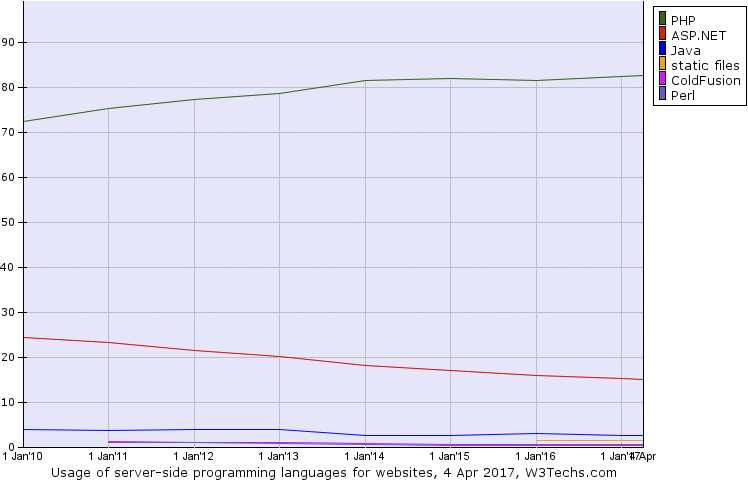
\includegraphics[width=0.9\textwidth]{server-side-languages.png}
    \caption{A graphic showing the global share of \emph{server-side programming languages} from January 2010 to April 2017. \emph{PHP} remains the dominant language with a share growing from 72.5\% to 82.6\% \cite{W3TechLanguageTrends}.}
    \label{fig:server-side-languages}
\end{figure}
%

% \paragraph{} % History of Content Management Systems.
The roots of the most well-known modern Content Management Systems (\emph{CMS}) date back to the early 2000s, when PHP was (and \emph{still is}) the dominant factor in terms of server-side programming languages (see Fig. \ref{fig:server-side-languages}). %% Please check, if reference is accurate enough

While the \emph{typical} CMS was starting out as mostly just a ``dynamic online tool'', it also shows that with seamlessly integrating new features gained through the development of its underlying programming languages, as well as steadily adding new functionalities (mostly requested by the community), a transition towards a fully-manageable and customizeable, semi-automatic web application was possible \cite[17]{dhillon2016}.

The advantages are clear: a web designer or content editor does not automatically have to be a web developer, who needs profound knowledge about software or server architecture. Instead, most of the time it is enough to know how to operate an FTP-client and to know the credentials of the built-in database service, submitted by the web hosting provider upon registration. As a summary, it can be said: \emph{Less people for less responsibilities}~--~the web application does the rest.

However, this progression also caused a few drawbacks, especially when it comes down to comparing the amount of workload needed before actually being able to create content for the World Wide Web. Due to the fact, that most CMSs evolved to their own sort of powerful admin panels, developers who are not keen about keeping their site updated, risk its defacing or other embarrassing attacks through unmanaged security holes in the code \cite[23]{dhillon2016}. So, how is it possible to bridge the gap between a fairly secure system and creating content whenever it is desired?

% \paragraph{} % Creating content using static HTML.
In 2008, \emph{Tom Preston-Werner} created \emph{Jekyll} out of his frustration of having the need of ``styling a zillion template pages'' and ``moderating comments all day long'' before even being ready to create content on his blogging engine \cite[]{PrestonWerner2008jekyll}. Furthermore he mentioned, that one of the other main reasons were the lack of possibility for publishing his posts on his own server, when subscribing to a fully-managed online hosting service like wordpress.com\footnote{\url{https://en.wordpress.com} -- a hosted version of Wordpress.}. Services like this offer only limited customization options, where there likely is no access to online storage and database without using the built-in admin panel. Even then, access might be very restricted.

The intended core functionality of Jekyll narrows down its mode of operation to handle three main components found in most static site generators today \cite[24]{dhillon2016}:

\begin{description}
  \item [Core language] -- The language a static generator is written in, for example JavaScript or Ruby.
  \item [Templates] -- The templating language to be used through the blog and posts.
  \item [Plug-ins] -- All static site generators allow for additional functionality through some
sort of a plug-in system.
\end{description}
In contrast to common dynamic CMSs, a static site generator outputs plain static HTML. It does it in a way, that a certain \emph{distribution} folder holds the complete web root, without the need of binding it to external services like databases or session management tools. Occasionally, different plug-ins also allow the generation of client-side \emph{JavaScript} or \emph{Cascading Style Sheet} files through their respective pre-processing tools.

\section{Jekyll}
\label{sec:jekyll}

As already explained, Jekyll was created out of the need for avoiding to service the blogging engine before writing and publishing content. Since it is deeply integrated into \emph{GitHub}, it is considered as the probably most-popular static site generator.

\subsection{History}
\label{sec:jekyll-history}
\emph{Tom Preston-Werner}, co-founder of GitHub\footnote{\url{https://github.com} -- GitHub Inc.}, announced it in October 2008 in one of his blog posts \cite{PrestonWerner2008jekyll}. Already in December 2008, it was introduced as build engine for the then newly featured GitHub Pages service, allowing owners of repositories to publish a static website by just pushing to a certain \emph{master} or \emph{gh-pages} branch \cite{PrestonWerner2008githubpages}, which is still available for free to this day.

All of this happened just 6 (respectively 8) months after GitHub was launched \cite{PrestonWerner2008githublaunch} and is now even being used by technology-leading companies to showcase their Open-Source efforts\footnote{\url{https://github.com/showcases/github-pages-examples} -- GitHub Pages examples.}.

\subsection{Technology}
\label{sec:jekyll-technology}
Jekyll was entirely written in \emph{Ruby}, as Tom Preston-Werner rather saw himself as a software developer in the first place, than as a content author \cite{PrestonWerner2008jekyll}. Until now, the repository for Jekyll still consists mainly of Ruby code at a share of roughly 77.5\%.

\subsubsection{Advantages}
One of the main advantages is the modular structure of its code base. By inheriting different Ruby classes, it is quite easy to extend and add features to fit the developer's needs. Due to its wide-spread usage initiated through the GitHub universe, Jekyll also has an accordingly huge user base and is therefore well documented \cite[26]{dhillon2016}.

Furthermore, its website\footnote{\url{http://jekyllrb.com} -- Jekyll website.}, which mainly acts as starting basis for documentation, is not only available as open-sourced git repository, it is also built using \texttt{Jekyll} to prove its universality.

Starting from scratch, the command \texttt{jekyll new my\_project} installs a blog environment for starters in the \texttt{./my\_project} folder. The basic install consists of an elementar blog post structure, \emph{Sass} source files, and a few template files written for Shopify's \emph{Liquid}\footnote{\url{https://help.shopify.com/themes/liquid} -- Shopify's Liquid template engine.} engine.\\
Using this starting environment, the unexperienced developer quickly gets a sufficient overview of what is generally possible using Jekyll, whereas the content author is able to fully concentrate himself on writing content, as the used \emph{Markdown} markup language requires little to no prior syntax knowledge. Furthermore, Jekyll already ships with a built-in webserver for quickly reviewing the rendered static output.

\subsubsection{Disadvantages}
As powerful as Ruby might be designed, many unskilled developers are facing difficulties right from the beginning, as most of them experience a steep learning curve. Nearly every single bit of customizing Jekyll requires Ruby knowledge, especially if it is desired to move along the ``predefined'' way and not including third-party extensions like \emph{Node.js} tools or else.

Additionally, its template language, Liquid, offers customization on a very high level, so it might happen to confuse business logic\footnote{How Jekyll processes data into programmatically readable structures.} with template logic\footnote{How Liquid transforms these structures into browser-readable HTML.}. To make things worse, different template constructions might also evolve over time and therefore causing a parallel coding universe when trying to surpass difficulties in the business logic.

%% bring some difficulties concerning ruby versions
%% ruby gems

\section{Hexo}
\label{sec:hexo}

\texttt{Hexo} understands itself as counterpart to \texttt{Jekyll}, mostly by covering the same ideas of static site generation, but building up completely on \texttt{Node.js}. It even offers a migration service for \texttt{Octopress}- and \texttt{Jekyll}-users who are willing to switch.

\subsection{History}
\label{sec:hexo-history}
\texttt{v1.0.0} was originally released in March 2013\footnote{\url{https://github.com/hexojs/hexo/releases/tag/1.0.0} -- Hexo v1.0.0 release page on \texttt{GitHub}.}, although development on \texttt{GitHub} dates back to September 2012 as the first commit was published using the message \emph{``init''}.

\emph{Tommy Chen}, its creator, first used \texttt{Octopress}\footnote{\url{http://octopress.org} -- Octopress website.} but quickly became dissatisfied with its performance, as the rendering of 54 blog posts already took more than a minute of compile time \cite{Chen2012hexodebut}. Since he assumed \texttt{Ruby} might be the cause for the lack of performance of his primarily used blogging framework, and further development on this case was not likely to happen any time soon, he decided to look for something which got his attention shortly before: \texttt{Node.js}.

However, \texttt{Node.js} was not really a big player back at that time, so the offer of blogging frameworks written in \texttt{JavaScript} was very dense and not really fitting the needs of \emph{Tommy Chen}. In his announcement article for \texttt{Hexo} \cite{Chen2012hexodebut}, he references a blog post of \emph{Boris Mann}, also an \texttt{Octopress} user at that time, listing a few \texttt{Node.js}-based blogging frameworks, which were already around in June 2012\footnote{\url{http://blog.bmannconsulting.com/node-static-site-generators} -- Blog article of \emph{Boris Mann} about \texttt{Node.js}-based blogging frameworks.}. Interestingly, only two of all the mentioned ones, \texttt{Wintersmith} and \texttt{DocPad} are still actively maintained today.

\subsection{Technology}
\label{sec:hexo-technology}
As already stated above, \texttt{Hexo} primarily consists of \texttt{JavaScript}, thus making it easier to start for developers with a front-end web development background. In fact, its \texttt{GitHub} repository shows \texttt{JavaScript} holding a share of 100\% on the source code\footnote{\url{https://github.com/hexojs/hexo} -- Hexo repository on \texttt{GitHub}.}.

\subsubsection{Advantages}
Right from the start, \texttt{Hexo} presents itself using its feature-rich command-line interface (\emph{CLI}), similar to \texttt{Jekyll}. Once it is installed, \texttt{hexo init my\_project} scaffolds a new starter template into the \texttt{./my\_project} folder.\\
As \emph{Tommy Chen} himself wanted an easy-to-use replacement for \texttt{Octopress}, \texttt{Jekyll} and \texttt{Hexo} share a lot of common features; their content files use both \texttt{YAML} frontmatter and \texttt{Markdown} by default, even the main configuration file uses a very similar structure in both frameworks. This should make it extremely easy switching from \texttt{Jekyll} to \texttt{Hexo}.

First and foremost, programming-unaware content authors might especially like its CLI, as it also offers to create files based on the \texttt{hexo new} command. Depending on other submitted command-line arguments, \texttt{Hexo} may automatically put the new post in the according sub-folder, whether it is a \emph{draft, page} or \emph{post}. Publishing a draft is as easy as \texttt{hexo publish}.\\
When creating content, \texttt{Hexo} also contains a feature-rich, \texttt{Octopress}-inspired custom tag selection for including content from \emph{YouTube, Vimeo} or \emph{GitHub Gists}.

Additionally, its plugin collection is also constantly growing and mostly community supported. A special naming convention using \texttt{hexo-} as prefix helps by determining which plugins to auto-load out of the \texttt{node\_modules} folder. Using this way, \texttt{Ruby's} \emph{convention over configuration} mantra is ported to \texttt{JavaScript} as well and supports especially beginners by not having to define the usage of a certain plugin.

\subsubsection{Disadvantages}
\texttt{Hexo} might look like as an ideal replacement for \texttt{Jekyll}, but since both share so much similarities, they also share some disadvantages. Whereas \texttt{Jekyll} ships with \emph{Liquid} and \emph{Sass} as standard, \texttt{Hexo} does with \emph{EJS} and \emph{Stylus}.\\
Although clearly stated, that both of these plugins might be easily uninstalled later on\footnote{\url{https://hexo.io/docs/setup.html\#package-json} -- Hexo's setup documentation.}, the whole setup pre-installation seems as opinionated as \texttt{Jekyll's}.

In addition to the already mentioned plugin system, a missing configuration option might as well turn out to be misleading in terms of customization options, especially when being dependent on the CLI. If customization is necessary, the developer often is forced to switch to the \texttt{JavaScript} API\footnote{\url{https://hexo.io/api/} -- Hexo's JavaScript API documentation.} or add a plugin to the project to make the build pipeline fit the customization's needs.

When it comes to caching, \texttt{Hexo} uses a homebrew version of \emph{JSON memory caching} called \texttt{Warehouse}, also created by \emph{Tommy Chen}\footnote{\url{https://github.com/tommy351/warehouse} -- Warehouse repository on \texttt{GitHub}.}, initially mentioned in the release notes of \texttt{3.2.0-beta.2} \cite{Chen2015hexorelease}. Using this plugin, a mode called ``Hot processing'' should enable faster re-builds. The main drawback here might be the caching speed, which is on the one hand filling up the memory when working on bigger projects, whereas the persisting of the database is fully dependent on file input/output write speeds of the underlying hard disk.\\
Furthermore, a constantly growing database file is hardly transferrable when trying to implement a decentralized building system out of \texttt{Hexo}.

\section{Metalsmith}
\label{sec:metalsmith}

Compared to the already described static site generators, \texttt{Metalsmith} is to be considered the youngest project.
It might also be the most radical project, as it was designed to consist of \textbf{nothing but plugins} \cite[31]{dhillon2016}. Therefore, in terms of still being a static site generator, it tries hard to push the limits much further than previously mentioned \texttt{Jekyll} and \texttt{Hexo}.

\subsection{History}
\label{sec:metalsmith-history}
Initially developed by \emph{Segment}\footnote{\url{https://segment.com} -- Segment's website.} for their internal needs, such as \emph{documentation, help} and \emph{blog pages} \cite{Metalsmith2015buildingblocks}, \texttt{Metalsmith} was finally open-sourced and made publicly available around February 2015 -- its commit history on \texttt{GitHub} dates back to February 4\textsuperscript{th}, 2014.\\
Most of the commits at that time were published by \emph{Ian Storm Taylor}, co-founder of \emph{Segment}, although his contribution to the project ends after releasing \texttt{v2.1.0} on September 24\textsuperscript{th}, 2015\footnote{\url{https://github.com/segmentio/metalsmith/commits/master?author=ianstormtaylor} -- Contributions of \emph{Ian Storm Taylor} to the Metalsmith repository on \texttt{GitHub}.} at the moment.

Like \texttt{Hexo}, \texttt{Metalsmith's} repository completely consists of \texttt{JavaScript} code, as its developers also were unsatisfied with the then existing static site generators. According to \emph{Chris Sperandio}, the \texttt{Metalsmith} developers desired pure flexibility for their ``wide array of use cases'', while other frameworks all asked for a certain structure on the content \cite{Metalsmith2015buildingblocks}.

\subsection{Technology}
\label{sec:metalsmith-technology}
Since \texttt{Metalsmith} consists of only plugins, specifically written for this very framework, there is no real standard setup provided. Although there are a few tutorials and best practices listed in its \texttt{GitHub} repository\footnote{\url{https://github.com/segmentio/metalsmith\#the-secret} -- Possibilities for using Metalsmith.}, as well as in a repository called ``\emph{awesome-metalsmith}''\footnote{\url{https://github.com/metalsmith/awesome-metalsmith} -- ``Awesome'' Metalsmith resources list.}, the initial dive-in might scare a few people away, since \texttt{Metalsmith} might not be as well documented as the previously mentioned frameworks. Moreover, most developers seem to experience a very steep learning curve at first, given the amount of customization options and the requirements for understanding the blog engine~infrastructure \cite[31]{dhillon2016}.

\subsubsection{Advantages}
Every developer is able to shape \texttt{Metalsmith} exactly to his/her needs, once he knows about the basic usage. It ships with a CLI, as well as a \texttt{JavaScript} API, where the ``real hacking'' is possible.\\
The CLI gets easily configured via a \texttt{metalsmith.json} file, stored in the project directory. It consists mainly of general project configurations, placed in the object's root, as well as an array of used plugins, respectively combined with their configuration.

It neither contains a pre-installed template engine, nor any other pre-processing tools, like \texttt{Sass} or \texttt{Less}. However, the available plugins support most of them to a satisfying extent. As an example, the \texttt{metalsmith-layouts} plugin is a wrapper for \texttt{consolidate.js}, which per se acts as a wrapper for the most common template engines\footnote{\url{https://github.com/tj/consolidate.js\#supported-template-engines} -- Consolidate.js-supported template engines on \texttt{GitHub}.}. Therefore, the developer is able to select the tools based on his/her preferences and may initialize a project from scratch, without needing to clean up any pre-installed demonstration files first.

Using the built-in \texttt{JavaScript} API, it is also possible to invoke the needed modules programmatically, which is one of the core topics of this Thesis.

\subsubsection{Disadvantages}
So much freedom in designing a project may also cause some dangers. In this case, one of the most crucial things is the arrangement of plugins in the configuration. Since \texttt{Metalsmith} acts as a streaming build system, every transformation of the content must happen at its time to not interfere with any upcoming plugins. This is especially important when a plugin might alter the underlying code in a way, that a following plugin becomes useless, as it might not be able to succeed in its predefined task. \emph{Andy Jiang} gives a good example about a sample structuring of \texttt{Metalsmith} plugins on the \emph{Segment} blog \cite{Metalsmith2015technicaldocumentation}.

As an example, the following code snippet shows one bold example of misconfiguration (See line no. 16):

%% Update line no. above, if code changes
\lstinputlisting[language=JavaScript]{chapters/02-state-of-the-art/_support/metalsmith.js}

%% Screenshot of npms.io for search query metalsmith static assets
\begin{figure}[b] % h-ere, t-op, b-ottom, p-age
    \centering
    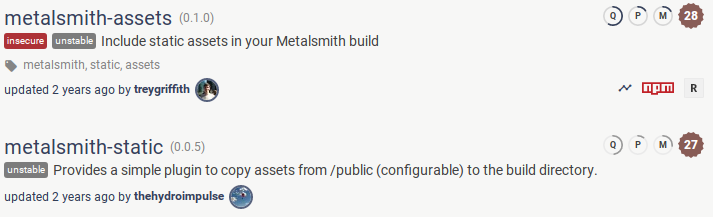
\includegraphics[width=0.9\textwidth]{metalsmith-static-plugins.png}
    \caption{A screenshot showing some of the results for the search query ``\emph{metalsmith static assets}'' on \url{https://npms.io}. Both of the shown entries describe an identical mode of operation within the \texttt{Metalsmith} build pipeline.\\
    Also notice the very unstable \texttt{semver} versions: \textbf{0.1.0} and \textbf{0.0.5}.}
    \label{fig:metalsmith-plugins}
\end{figure}
%

Moreover, the available plugins may seem as not as popular as the plugins from \texttt{Hexo}, given the average amount of stars received on \texttt{GitHub}. This might be due to the often missing maintainance, or simply because of the fact, that there seem to be multiple plugins for one single task (See Fig. \ref{fig:metalsmith-plugins}).

\section{Comparison}
\label{sec:comparison}

To conclude the summaries of different static site generators, a short overview using a table is given below (see Table \ref{table:comparison}). The comparison is built up on advantages and disadvantages, as well as the most important features they consist of. Therefore overall popularity and customizability play an as important role, as the language they are written in. However, Metalsmith stands a little bit out, as it does not provide a full-featured framework -- it merely serves as the basis for further plugin setup, whereas Jekyll and Hexo already contain some sort of standard setup.
The numbers of plugins in Table \ref{table:comparison} were taken from search queries on \url{https://npms.io} and \url{https://rubygems.org}.

\begin{table}
  \caption{A comparison of static site generators}
  \label{table:comparison}
  \centering
  \setlength{\tabcolsep}{5mm}
  \def\arraystretch{1.25}
  \begin{tabular}{|r||c|c|c|}
    \hline
    & \emph{Jekyll} & \emph{Hexo} & \emph{Metalsmith} \\
    \hline
    \hline
    Language & Ruby & JavaScript & JavaScript \\
    \hline
    Foundation & Oct. 2008 & Sept. 2012 & Feb. 2014 \\
    \hline
    Contributors & \textasciitilde 700 & \textasciitilde 100 & \textasciitilde 50 \\
    \hline
    Plugins & \textasciitilde 800 & \textasciitilde 600 & \textasciitilde 590 \\
    \hline
    Customizability & Mediocre & Low & High \\
    \hline
    Opinionatedness & High & High & Low \\
    \hline
    Standard templates & Liquid & Swig & \emph{none} \\
    \hline
  \end{tabular}

\end{table}

